\chapter{选课指导}
\section{课程分类}
\subsection{北京大学课程分类}

详情见开学期间会发放的《北京大学本科生选课手册》和《工学院本科教学手册》，这两份文件极其重要，请务必仔细研究。毕业之前，必须修完的学分（见以上两份文件）约为140学分，不同的专业和方向毕业学分要求不同\footnote{也就是说，修完这些学分和对应课程是你拿毕业证书的必然要求，但这并不代表你只能选这些课，在力所能及的范围内选修感兴趣的课程也是可以的}，下面列举了部分课程\footnote{仅代表往年情况，26级具体情况不太一样，如计概只有python班，数算被改为人工智能与算法设计}：

\begin{figure}[htbp]
	\centering
	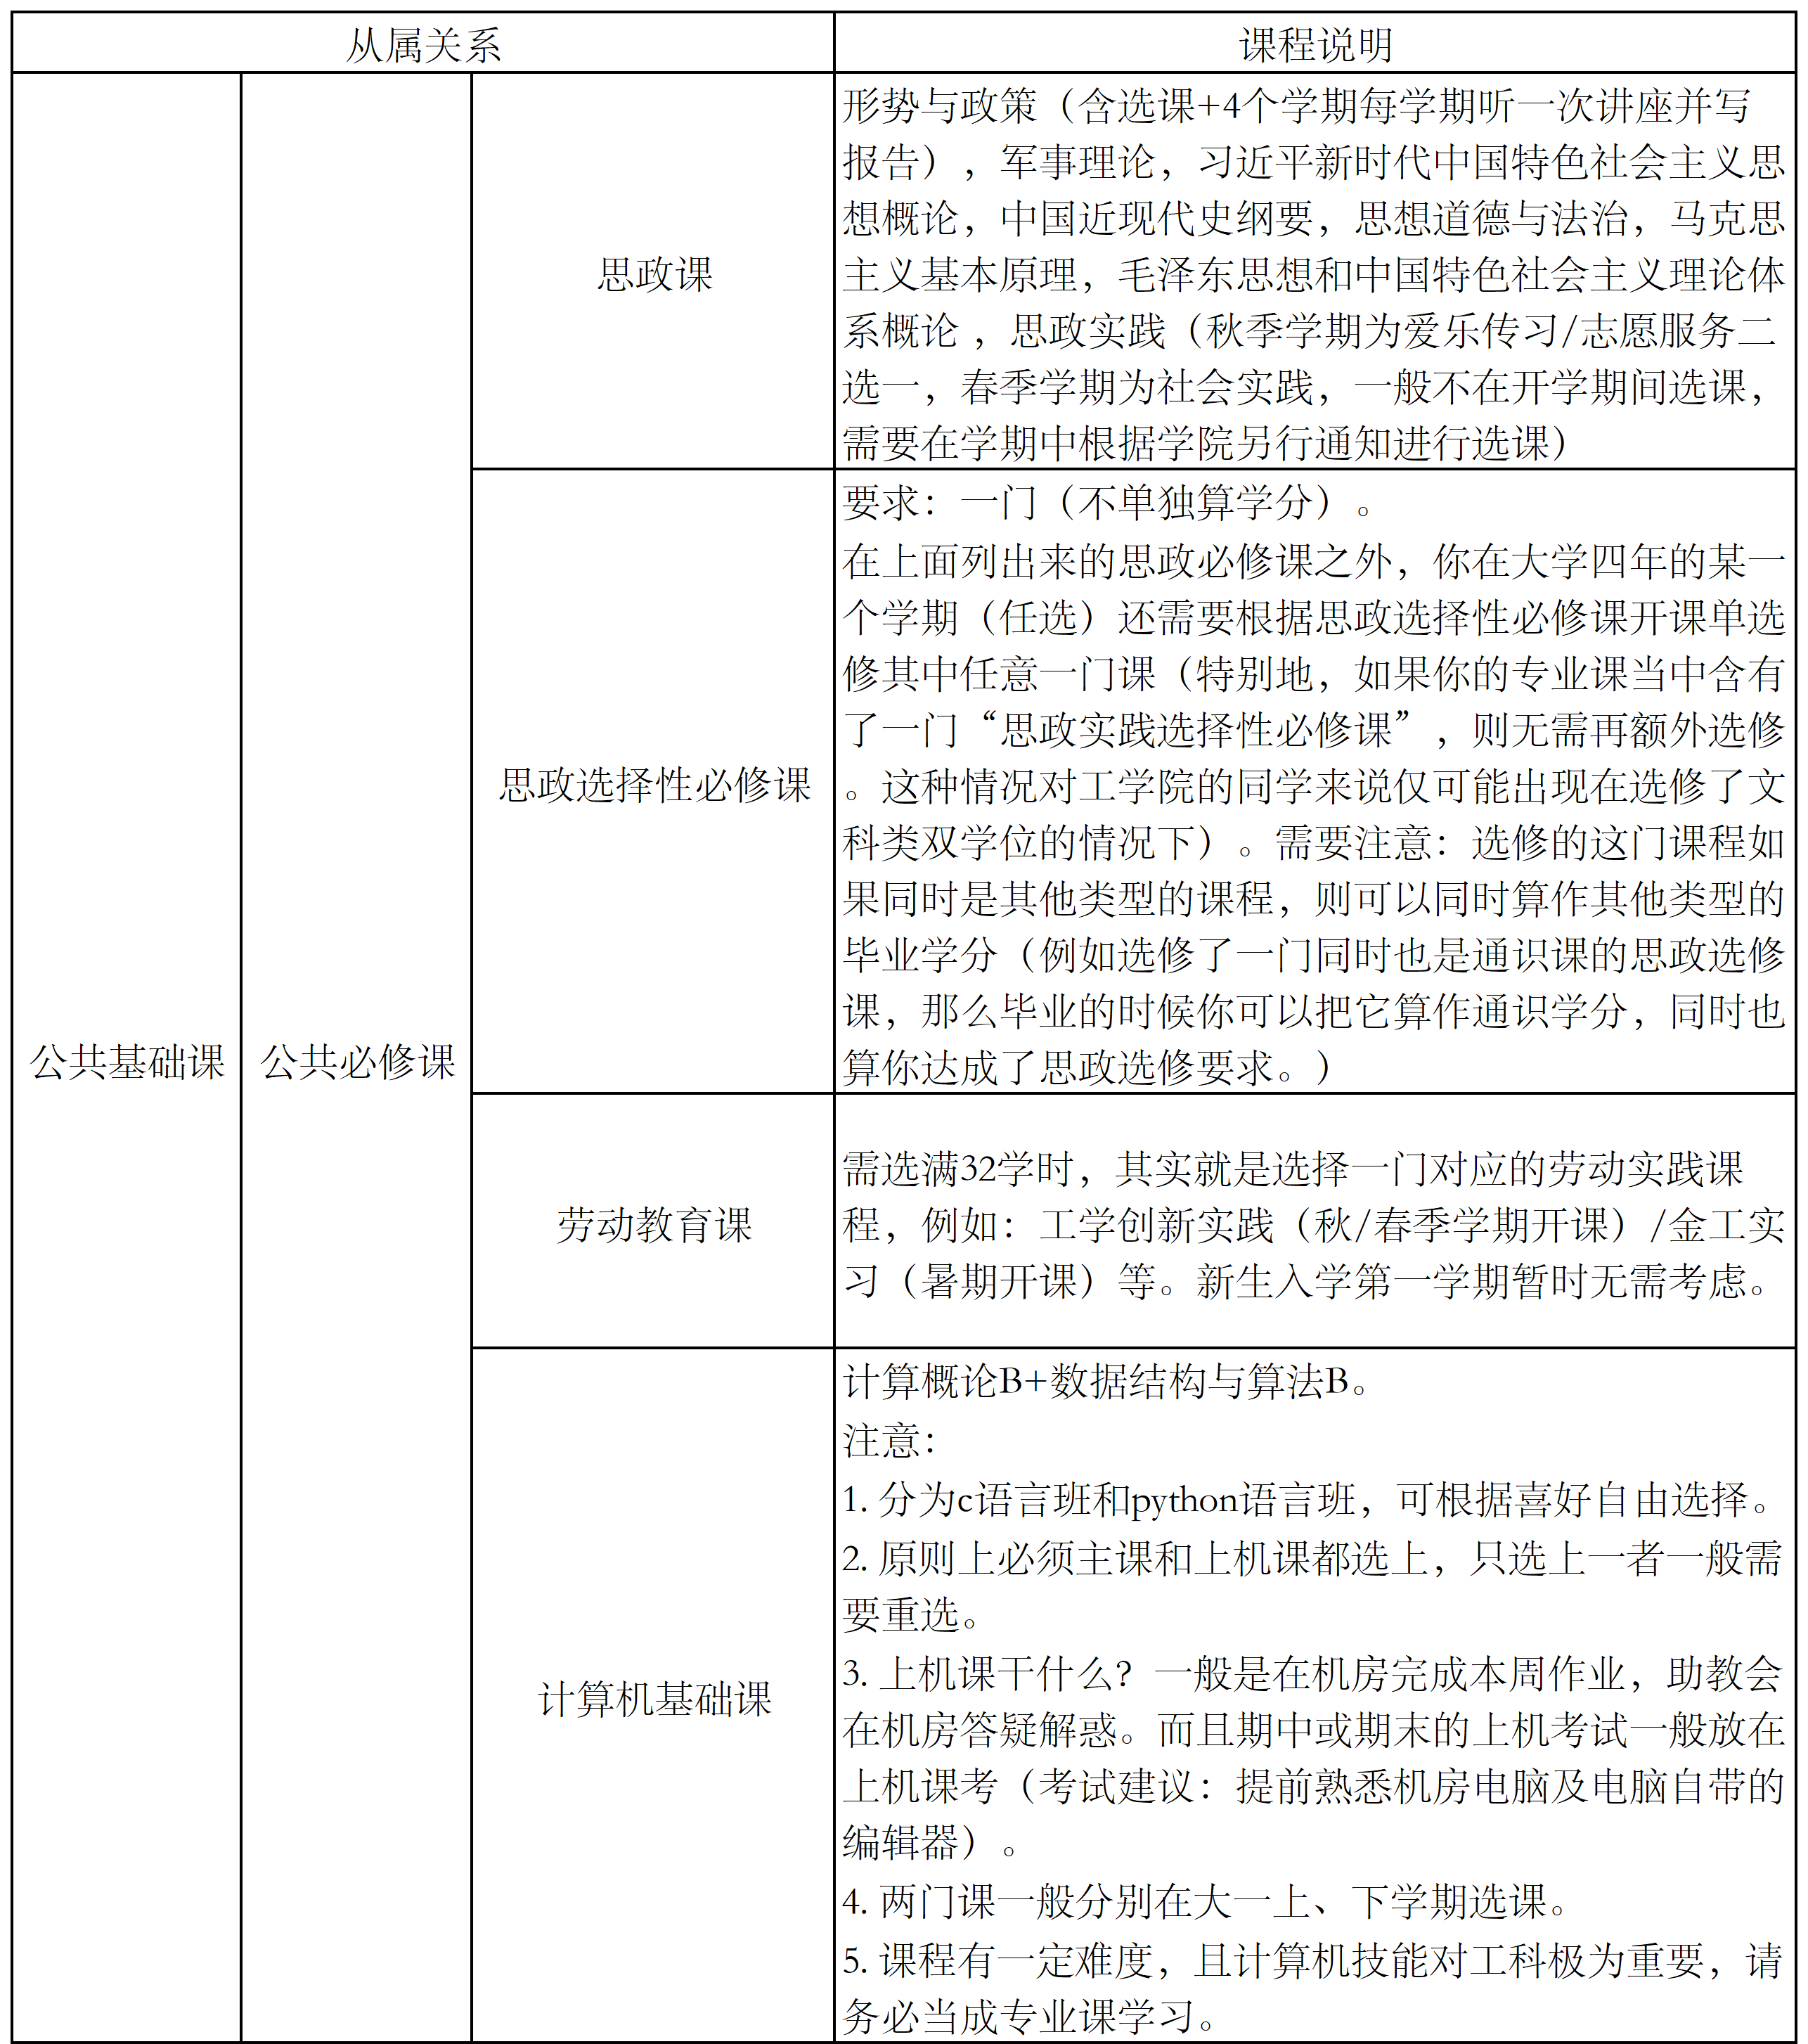
\includegraphics[width=1.02\linewidth]{assets/大表1.png}
\end{figure}

%%%%%%%%%%%%%%%%%%%%%%%%%%这里有个大表格
\begin{figure}[H]
	\centering
	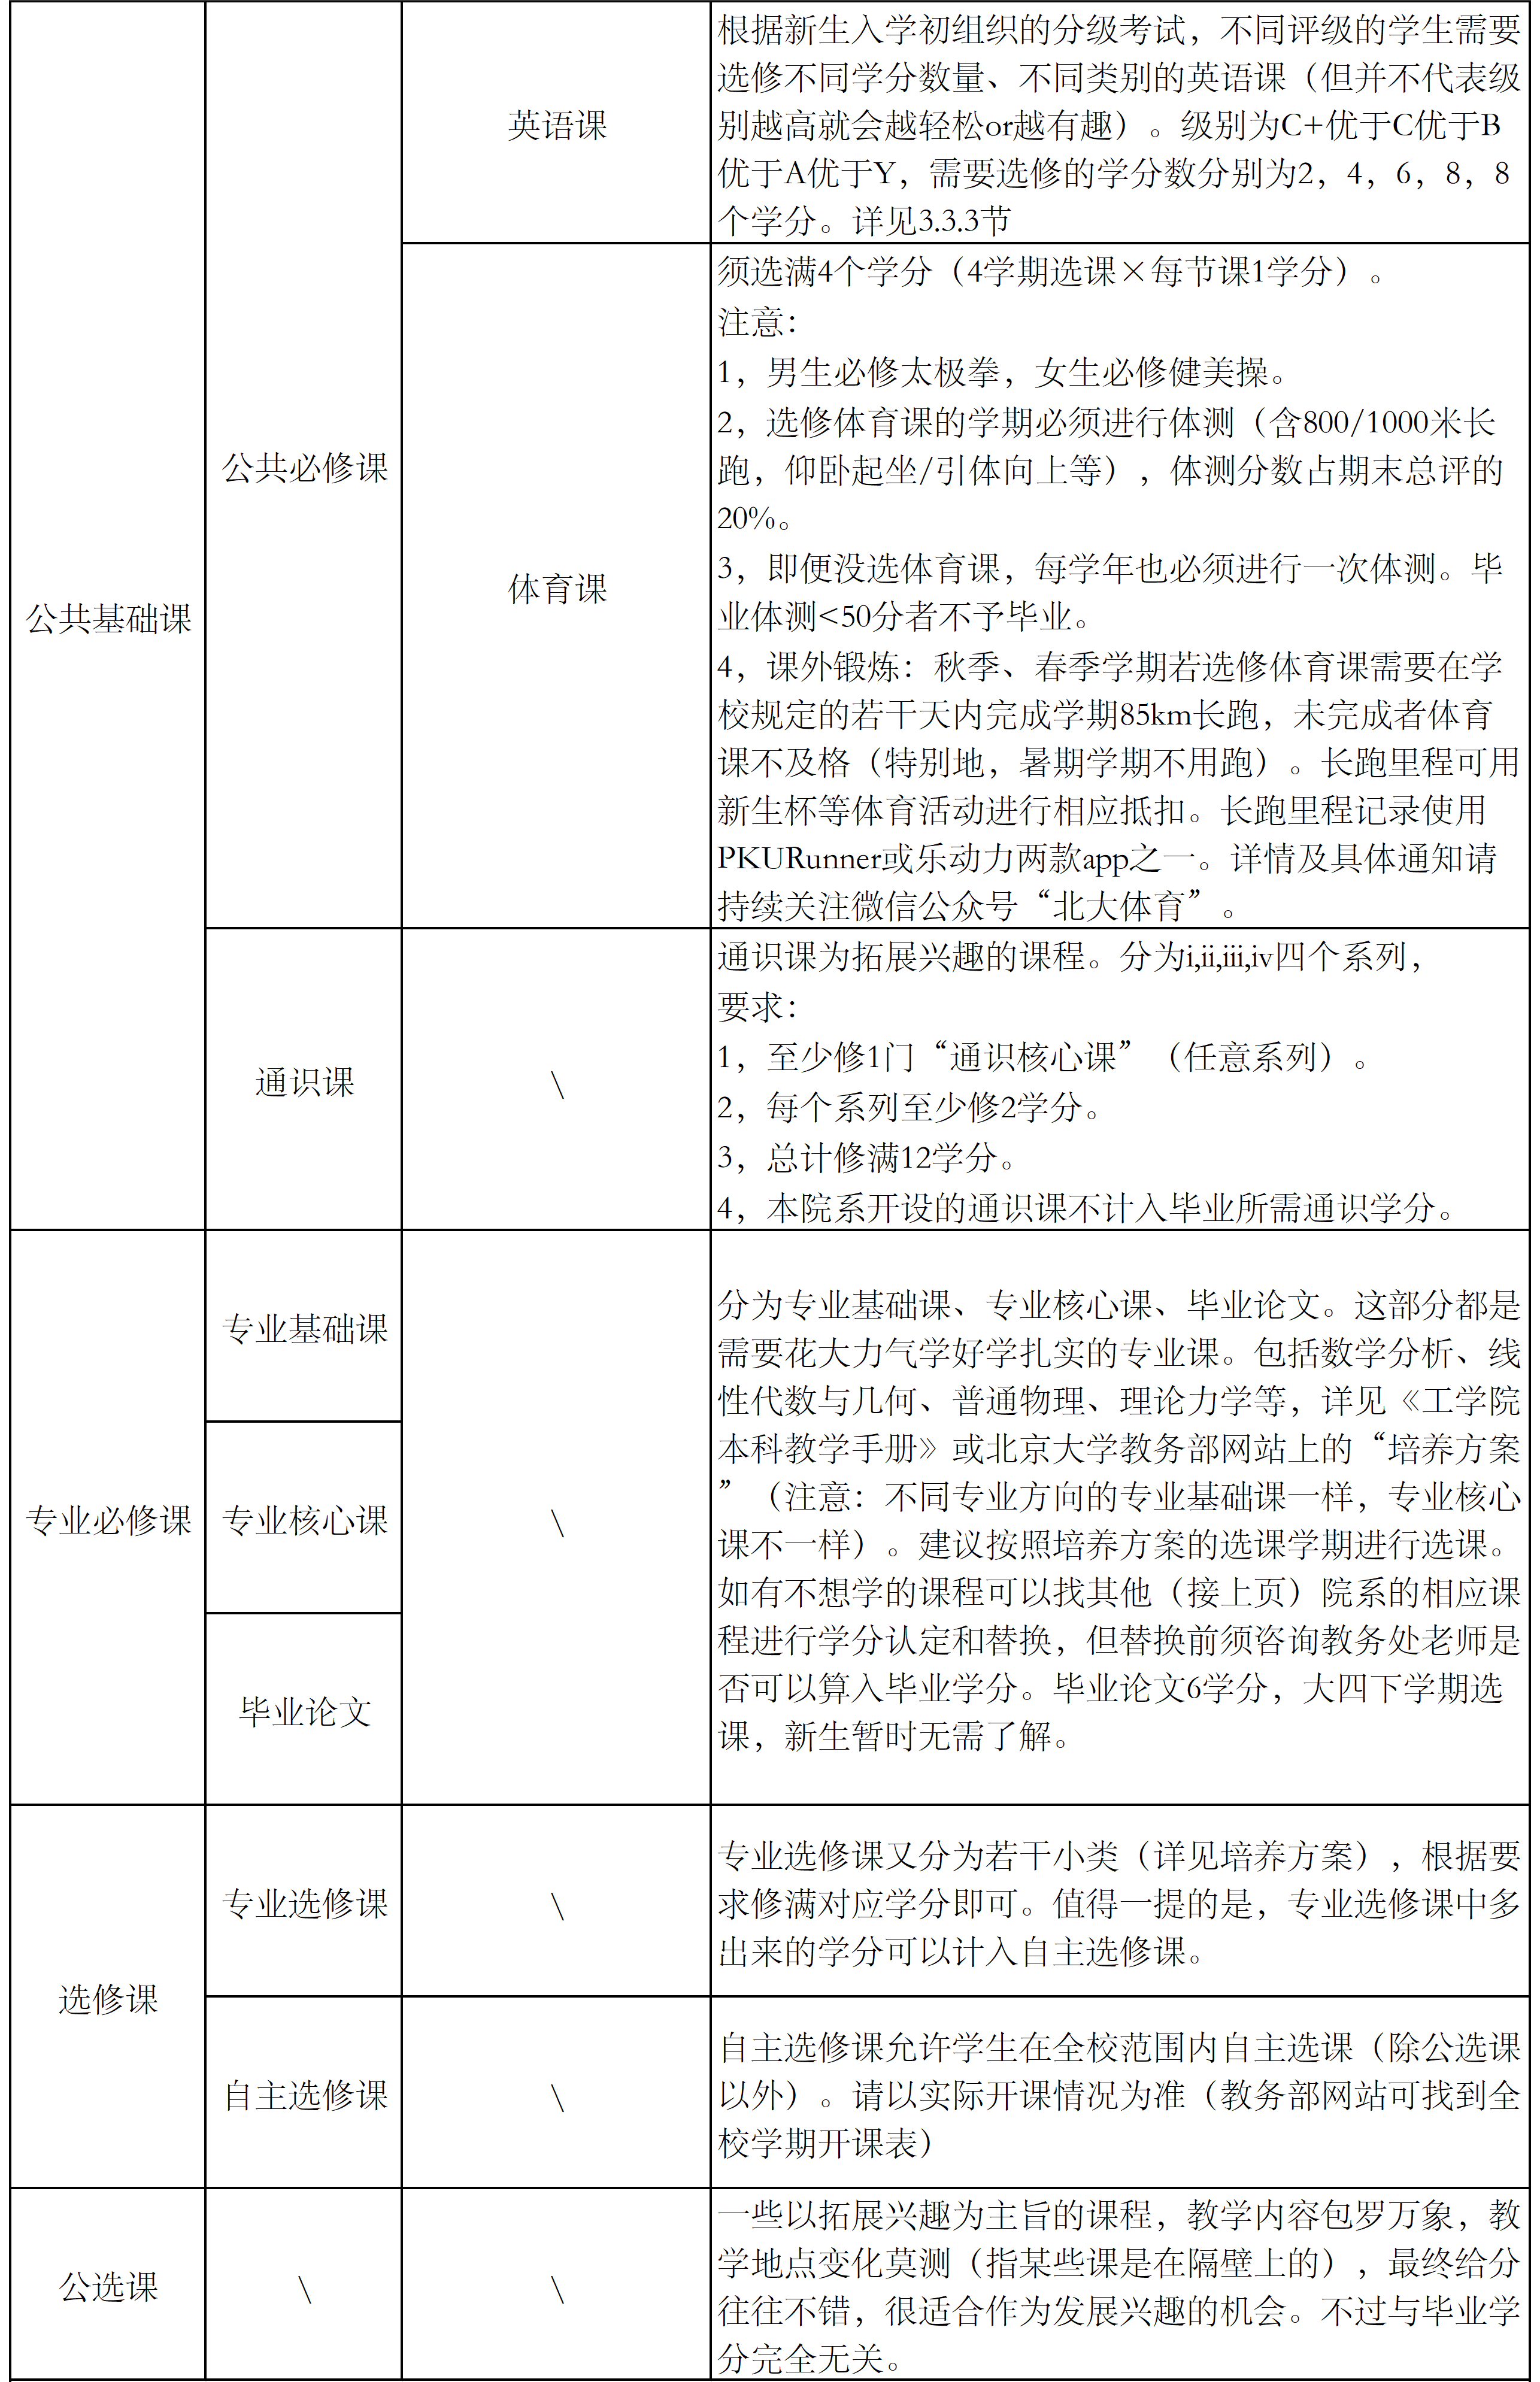
\includegraphics[width=1.02\linewidth]{assets/大表2.png}
\end{figure}



总结：
\begin{figure}[H]
	\centering
	
\includegraphics[width=0.2\linewidth]{assets/2.1.1衡量.png}
\end{figure}

\section{毕业要求}
1. 毕业要求：

修完培养方案中要求的学分，或经教务部审核认定的可以转化的学分。

\vspace{10pt}

2. 推免（保研）要求：

原则上在大三前修完专业必修课和大部分专业选修课，各专业存在差异，详见培养方案。强基和非强基同学要求有所不同，详见1.2.2节

\vspace{10pt}

该部分仅为获得免试研究生资格的必要条件而非充分条件，录取要求请见招生单位相关规定。各专业、各录取单位存在差异，详见培养方案。

3. 荣誉学位要求：

考虑政策变化，具体请参考学院评定细则。

\section{选课网基本操作}

欲进入选课系统，可从北京大学个人门户进入，也可在搜索引擎直接搜索“北京大学选课系统”。下面将以时间为主要线索，对北京大学选课系统（海淀大赌场doge）进行简要说明。

选课总体上分为五个阶段，分别是\textbf{\textbf{预选、补退选第一阶段、补退选第二阶段、补退选第三阶段、补选}}。又可以简单地根据预选抽签前后把时间划分为两个阶段，前一个大阶段（预选）是主要\textbf{\textbf{选课}}阶段，后一个大阶段（补退选和补选）是主要\textbf{\textbf{抢课}}阶段。

\vspace{10pt}

整体时间轴（具体日期每年不同，需要关注教务通知，尤其是暑假学期选课）以2026年秋季学期为例：
\begin{figure}[htbp]
	\centering
	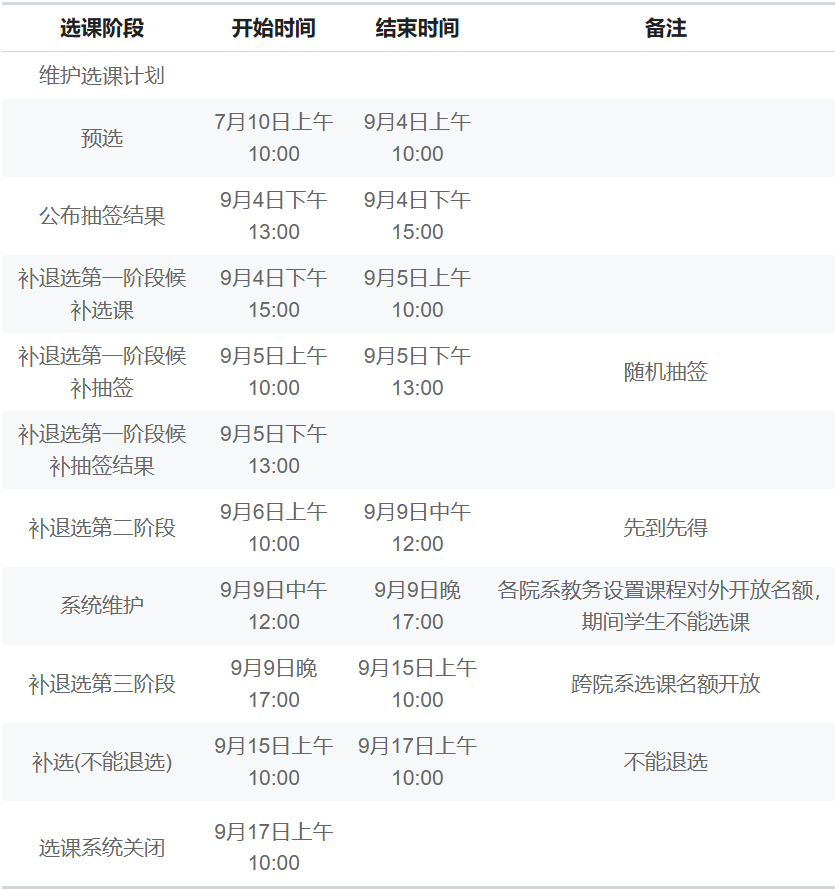
\includegraphics[width=0.6\linewidth]{assets/选课时间轴.png}
	\renewcommand{\figurename}{图}
	\caption{2026年秋季学期选课时间轴}
	\label{fig:enter-label}
\end{figure}

\vspace{10pt}

\textbf{1. 预选}

(1)把课程从选课列表（货架）添加到选课计划（购物车）。

教务会将一些重要课程提前加入选课计划。课程加入选课计划后还没有成功预选。点击课程名称，可以获悉课程简介、所用课本、课程大纲等信息。不过很多信息并不完全准确（有的甚至是十几年之前写的版本），具体内容务必咨询开课老师、学长学姐们。

\vspace{10pt}

(2) 把选课计划（购物车）中的课程添加到预选单（待“支付”）中。

\vspace{10pt}

(3) 为预选课程投点（详见2.5.1节）。

\vspace{10pt}

(4) 等待抽签结果，查看课程是否成功选上。

\vspace{10pt}

\textbf{2. 补退选第一阶段}

从此阶段开始，选课操作需要手动填写验证码以防作弊，每次选课或刷新后均需要填写。

\vspace{10pt}

(1) 如果有人退课，会让出该课程的若干名额，在课程栏显示为xx/xx。

\vspace{10pt}

(2) 把课程加入补退选单中，具体操作和预选阶段基本相同。

\vspace{10pt}

(3) 等抽签抢空出的名额。通常而言几率不大，常常是几十个人抢几个名额。需要提醒的是，教务在补退选第一阶段扩充的名额，会在时间截止前显示在课程栏中。若临近截止时间仍未显示，则大概率不会再扩充名额。

\vspace{10pt}

\textbf{3. 补退选第二阶段}

抢课最关键的阶段，\textbf{先到先得，不抽签}。

\vspace{10pt}

(1) 蹲点等其他同学退课，刷新选课网站以获得空余名额。退课和名额刷新往往不会同步。

\vspace{10pt}

(2) 拼手速抢！具体操作和预选阶段基本相同。

\vspace{10pt}

\textbf{4. 补退选第三阶段}

\vspace{10pt}

(1) 跨院系选课名额开放，可以选一些其他院系的课程。该阶段对于有志于转专业的同学来说比较重要。

\vspace{10pt}

(2) 抢课规则同3。

\vspace{10pt}

\textbf{5. 补选}

\vspace{10pt}

(1) 该阶段选中某一课程后不可退选。

\vspace{10pt}

(2) 可以恳求开课老师收留，或者恳求教务老师增加选课名额。该方法需要灵活使用。

\vspace{10pt}

\textbf{6. 投点技巧}

此处介绍选课投点技巧\footnote{虽然并不是很重要}。

\vspace{10pt}

每位同学一共有99点意愿值，需要在不同课程之间分配。对同一门课程而言，在其他条件均相同的前提下，投点越多的同学，选中该门课程的概率越大。当然，若课程特别火爆，则可能有99意愿值仍然失利的非酋；反之，也可能有0意愿值上岸的超级欧皇。那么，我们该怎样分配点数呢？这时我们需要考虑两个问题：\textbf{什么课程需要投点；投点的课程要投多少点}。

\vspace{10pt}

\textbf{什么课程需要投点：}

\vspace{10pt}

我们已知，对于专业课，比如理论力学方向大家一定要学的数学分析（一），开放名额一定大于对应年级的总人数；且无论如何，教务老师会保证同学们选上本专业的专业课。那么，这门课完全没有投点的必要——事实上系统中也投不了点，因为专业课等会被设置为系统推荐课程，无需投点。什么课需要投点？答案是各类供不应求的体育、通识、英语、政治等。

\vspace{10pt}

我们又知道，一般而言，每位同学每学期最多可以选25学分的课程。这其中专业课占了很大一部分。这就导致了一个问题：若某位同学想预选多门通识课作为备选项，但是发现无法将所有备选项加入预选，否则会超过学分上限。这时可以如下取巧：在预选阶段，不选之后一定会选上的专业课，用专业课的学分空档预选那些通识课备选项。待选上心仪的通识课后，把其他没选上的备选课退掉，再在补退选阶段把专业课加回来。这是一种小技巧，更多技巧建议自行体悟。

\vspace{10pt}

\textbf{该课程投多少点：}

\vspace{10pt}

比较热门的投点办法有两个：质数投点法（玄学）和all-in投点法。前者认为，只要所有投点都是质数，则最终选课成功率大大上升。后者不计代价地把大量点数\footnote{甚至所有点数}砸到一门课中，以期待高概率选中一门课。

\vspace{10pt}

后一种方法未必不好，因为这至少保证了一门好课大概率选中。当然，也有可能all-in但仍然选不上orz。如果我们采取平均投点的办法，每门课选中概率都不大，有可能出现所有课全都选不上的情况，但也有可能全中。最终的投点办法，还需自行衡量。有一个有意思但未必有用的投点辅助程序可以玩一下。\href{https://wyjjmzx.github.io/pku/toudian.html}{https://wyjjmzx.github.io/pku/toudian.html}

\section{选课信息来源}
我们常用以下途径判断一个课程的综合好评率：

\vspace{10pt}

1.在选课网的“选课计划”中，点击课号或课名，可以查看课程的先修课程、简介、大纲、教学评估得分等信息。其中教学评估是每位同学在临近期末考试时给课程做出的评估。选课网上的信息主要来自老师、助教、教务等，相对注重课程的内容部分，也更正式，而以下四种渠道的信息则更多来自同学。

\vspace{10pt}

2. 看“预选名额/计划名额”。本质上是直接应用他人劳动成果。其他同学搜索了解该课程后觉得不错，因此预选人数较多，那大概率这门课的综合口碑不错。

\vspace{10pt}

3. 树洞treehole.pku.edu.cn，搜索课程简写或老师姓名简写即可查到学长学姐的课程测评。考虑到树洞的匿名性质，课程评测等内容需要同学们注意分辨。

\vspace{10pt}

4. 非官方课程测评网站。在搜索引擎中直接搜索“北大课程测评”，第一个网站即为课程测评网站。该网站完全非官方，且完全不控评，内容同样地需要同学们注意分辨。

\vspace{10pt}

5. 广泛咨询靠谱的学长学姐，获得较为详细的听课感受等信息。

\vspace{10pt}

\textbf{核心要义：不仅仅追求良好的给分，更要追求自身兴趣能力的发展。}

\section{特殊选课模式}
\subsection{跨院系选课}
有志于转专业、双专业、辅修的同学需要注意，其他院系的专业课只可在补退选第三阶段进行选择。因此，需要提前为想选的课预留出时间和学分空间。

\vspace{10pt}

如果没有转专业、双专业、辅修打算，也可以在这一环节选择其他院系感兴趣的课程。学分可计入毕业学分中的“自主选修课”部分。

\subsection{课程替代}
培养方案是灵活机动的。根据培养方案，一些课程之间可以互相替代，进行毕业学分认定。关于培养方案上未明确的内容，请主动咨询工学院教务老师。

\subsection{冲突选课和手工选课}
申请特别麻烦，且一般用不上。若实在需要可参照：教务部网站-学生-选课和退课。

\subsection{双学位选课与超学分选课}
分为主修+辅双两个选课通道。辅双通道可以进行双专业、辅修课程的选择，且无需投点。通过辅双通道选择的双学位课程需要缴纳相应学费\footnote{详见本手册4.1}。

\vspace{10pt}

理论上，每学期选课量为14$\sim$25学分。当挂科不超过两门时，可以申请超学分选课，一般至多为每学期30学分。超学分选课需要经历一系列申请、审批过程，详见教务部官网。

\vspace{10pt}

特别地，双专业学生选课每学期学分上限为30学分。

\subsection{中期退课}
每学期中期\footnote{第八周左右}可根据教务通知进行中期退课。

\vspace{10pt}

体育课，第10周之前已经结束的课程，以及物理、生物、化学类实验课不允许中期退课。因病等特殊情况需要退体育课的同学，须提供由任课教师以及体育教研部主管教学的领导签字同意的《北京大学本科生手工退课申请表》，在退课期间交至体育教研室教务办公室（五四体育中心203），逾期将不予受理。

\vspace{10pt}

退课后，成绩单上该课程记为W，不参与绩点计算。退课后每学期所修学分一般不得低于14学分下限。

\vspace{10pt}

中期退课是某一门课程实在学不下去时的应急策略。过多的中期退课可能会让老师对学生的能力产生质疑。同学们可以适当使用，但不建议过度依赖。

\subsection{绩点改革}
以下内容依据教务部《关于进一步做好本科学业评价工作的通知》。该文件发布于2025年7月25日。

\vspace{10pt}

改革的具体影响如下：

\vspace{10pt}

1.从2025年秋季学期开始，每学期第九周结束前，同学们可在部分公共基础课程和专业课程包以外的课程内选择1门课，以“合格制（P/NP）”方式记载成绩。

\vspace{10pt}

2.允许课程等级制给分，取消课程优秀率限制。

\vspace{10pt}

3.从2025级开始，在各项含有学业评价的工作中不再使用绩点，而使用完整成绩单。

\vspace{10pt}

其中，笔者认为有几点需要着重：

\vspace{10pt}

1.百分制成绩与等级制成绩没有直接转换关系。

\vspace{10pt}

2.部分公共基础课程（包括大学英语、思想政治理论必修课、信息课程、军事理论、体育课），主修专业的专业必修课及院系特定课程不得采用P/NP方式记载成绩。也就是说，大一的大家可以选择P/NP方式的课程主要是通识课。

\vspace{10pt}

3.更关注于专业课的成绩排名。

\vspace{10pt}

4.如果按均分制计分，相比绩点制来说，低分课程的影响没那么大（绩点制下，任何一门<70分的课程对绩点都是灾难性打击）

\subsection{不按照培养方案选课}
理论上，同学们可以有自己的选课规划。但需要指出的是，培养方案的设置有很大的合理性，适合绝大多数人的学习进程。如果想按照自己的节奏安排课程，建议与老师、学长学姐深入探讨一下这种方案的合理性。
